
%package list
\documentclass{article}
\usepackage{amsmath}
\usepackage[top=3cm, bottom=3cm, outer=3cm, inner=3cm]{geometry}
\usepackage{multicol}
\usepackage{graphicx}
\usepackage{url}
%\usepackage{cite}
\usepackage{hyperref}
\usepackage{array}
%\usepackage{multicol}
\newcolumntype{x}[1]{>{\centering\arraybackslash\hspace{0pt}}p{#1}}
\usepackage{natbib}
\usepackage{pdfpages}
\usepackage{multirow}
\usepackage[normalem]{ulem}
\useunder{\uline}{\ul}{}
\usepackage{svg}
\usepackage{xcolor}
\usepackage{listings}
\lstdefinestyle{ascii-tree}{
    literate={├}{|}1 {─}{--}1 {└}{+}1 
  }
\lstset{basicstyle=\ttfamily,
  showstringspaces=false,
  commentstyle=\color{red},
  keywordstyle=\color{blue}
}
%\usepackage{booktabs}
\usepackage{caption}
\usepackage{subcaption}
\usepackage{float}
\usepackage{array}

\newcolumntype{M}[1]{>{\centering\arraybackslash}m{#1}}
\newcolumntype{N}{@{}m{0pt}@{}}


%%%%%%%%%%%%%%%%%%%%%%%%%%%%%%%%%%%%%%%%%%%%%%%%%%%%%%%%%%%%%%%%%%%%%%%%%%%%
%%%%%%%%%%%%%%%%%%%%%%%%%%%%%%%%%%%%%%%%%%%%%%%%%%%%%%%%%%%%%%%%%%%%%%%%%%%%
\newcommand{\itemEmail}{ccapatinta@unsa.edu.pe}
\newcommand{\itemStudent}{Capatinta Almanza Camilo B. A.}
\newcommand{\itemCourse}{Lab. Análisis y Diseño de Algoritmos}
\newcommand{\itemCourseCode}{1702231}
\newcommand{\itemSemester}{IV}
\newcommand{\itemUniversity}{Universidad Nacional de San Agustín de Arequipa}
\newcommand{\itemFaculty}{Facultad de Ingeniería de Producción y Servicios}
\newcommand{\itemDepartment}{Departamento Académico de Ingeniería de Sistemas e Informática}
\newcommand{\itemSchool}{Escuela Profesional de Ingeniería de Sistemas}
\newcommand{\itemAcademic}{2026 - B}
\newcommand{\itemInput}{10/09/2026}
\newcommand{\itemOutput}{14/09/2026}
\newcommand{\itemPracticeNumber}{02}
\newcommand{\itemTheme}{Ordenamiento: Insertion Sort, Selection Sort}
%%%%%%%%%%%%%%%%%%%%%%%%%%%%%%%%%%%%%%%%%%%%%%%%%%%%%%%%%%%%%%%%%%%%%%%%%%%%
%%%%%%%%%%%%%%%%%%%%%%%%%%%%%%%%%%%%%%%%%%%%%%%%%%%%%%%%%%%%%%%%%%%%%%%%%%%%

\usepackage[english,spanish]{babel}
\usepackage[utf8]{inputenc}
\AtBeginDocument{\selectlanguage{spanish}}
\renewcommand{\figurename}{Figura}
\renewcommand{\refname}{Referencias}
\renewcommand{\tablename}{Tabla} %esto no funciona cuando se usa babel
\AtBeginDocument{%
	\renewcommand\tablename{Tabla}
}

\usepackage{fancyhdr}
\pagestyle{fancy}
\fancyhf{}
\setlength{\headheight}{40.51407pt}
\renewcommand{\headrulewidth}{1pt}
\renewcommand{\footrulewidth}{1pt}
\fancyhead[L]{\raisebox{-0.2\height}{
\includegraphics[width=3cm]{img/logo_episunsa.png}}}
\fancyhead[C]{\fontsize{7}{7}\selectfont	\itemUniversity \\ \itemFaculty \\ \itemDepartment \\ \itemSchool \\ \textbf{\itemCourse}}
\fancyhead[R]{\raisebox{-0.2\height}{
\includegraphics[width=1.2cm]{img/logo_abet}}}
\fancyfoot[L]{Estudiante Capatinta C.}
\fancyfoot[C]{\itemCourse}
\fancyfoot[R]{Página \thepage}

% para el codigo fuente
\usepackage{listings}
\usepackage{color, colortbl}
\definecolor{dkgreen}{rgb}{0,0.6,0}
\definecolor{gray}{rgb}{0.5,0.5,0.5}
\definecolor{mauve}{rgb}{0.58,0,0.82}
\definecolor{codebackground}{rgb}{0.95, 0.95, 0.92}
\definecolor{tablebackground}{rgb}{0.8, 0, 0}

\lstset{frame=tb,
	language=bash,
	aboveskip=3mm,
	belowskip=3mm,
	showstringspaces=false,
	columns=flexible,
	basicstyle={\small\ttfamily},
	numbers=none,
	numberstyle=\tiny\color{gray},
	keywordstyle=\color{blue},
	commentstyle=\color{dkgreen},
	stringstyle=\color{mauve},
	breaklines=true,
	breakatwhitespace=true,
	tabsize=3,
	backgroundcolor= \color{codebackground},
}

\begin{document}
	
	\vspace*{10px}
	
	\begin{center}	
		\fontsize{17}{17} \textbf{ Informe de laboratorio \itemPracticeNumber}
	\end{center}
	\centerline{\textbf{\Large Tema: \itemTheme}}
	%\vspace*{0.5cm}	

	\begin{flushright}
		\begin{tabular}{|M{2.5cm}|N|}
			\hline 
			\rowcolor{tablebackground}
			\color{white} \textbf{Nota}  \\
			\hline 
			     \\[30pt]
			\hline 			
		\end{tabular}
	\end{flushright}	

	\begin{table}[h!]
		\begin{tabular}{|x{4.7cm}|x{4.8cm}|x{4.8cm}|}        
			\hline 
			\rowcolor{tablebackground}
			\color{white} \textbf{Estudiante} & \color{white}\textbf{Escuela}  & \color{white}\textbf{Asignatura}   \\
			\hline 
			{\itemStudent \par \itemEmail} & \itemSchool & {\itemCourse \par Semestre: \itemSemester \par Código: \itemCourseCode}     \\
			\hline 			
		\end{tabular}
	\end{table}		
	
	\begin{table}[H]
		\begin{tabular}{|x{4.7cm}|x{4.8cm}|x{4.8cm}|}
			\hline 
			\rowcolor{tablebackground}
			\color{white}\textbf{Laboratorio} & \color{white}\textbf{Tema}  & \color{white}\textbf{Duración}   \\
			\hline 
			\itemPracticeNumber & \itemTheme & 04 horas   \\
			\hline 
		\end{tabular}
	\end{table}
	
	\begin{table}[H]
		\begin{tabular}{|x{4.7cm}|x{4.8cm}|x{4.8cm}|}
			\hline 
			\rowcolor{tablebackground}
			\color{white}\textbf{Semestre académico} & \color{white}\textbf{Fecha de inicio}  & \color{white}\textbf{Fecha de entrega}   \\
			\hline 
			\itemAcademic & \itemInput &  \itemOutput  \\
			\hline 
		\end{tabular}
	\end{table}
	
	\section{Ejercicios/Problemas propuestos }
	
	\subsection{Ejercicio 1}

        Antes de resolver los ejercicios propuestos, compilen y ejecuten en su computadora el código de Insertion Sort y Selection Sort mostrado en la Sección II. Cámbienlo por un arreglo de datos propio (mínimo 8 elementos) y verifiquen que el resultado ordenado sea correcto. Esto les ayudará a comprobar que entienden cómo funciona cada algoritmo antes de continuar.

    \lstinputlisting[language=c++, caption={Ejercicio 01: InsertionSort y SelectionSort con más datos},numbers=left,]{../ejerciciosPropuestos/e1.cpp}

    \begin{itemize}
        \item Se prueban InsertionSort y SelectionSort con un array de igual tamaño y de mismos datos, llegando ambos al mismo resultado pero 
		con tiempos diferentes, siendo más eficiente SelectionSort porque demoró menos tiempo. Aunque esto puede cambiar en diferentes contextos y situaciones. 
    \end{itemize}

    \begin{figure}[H]
    \centering
    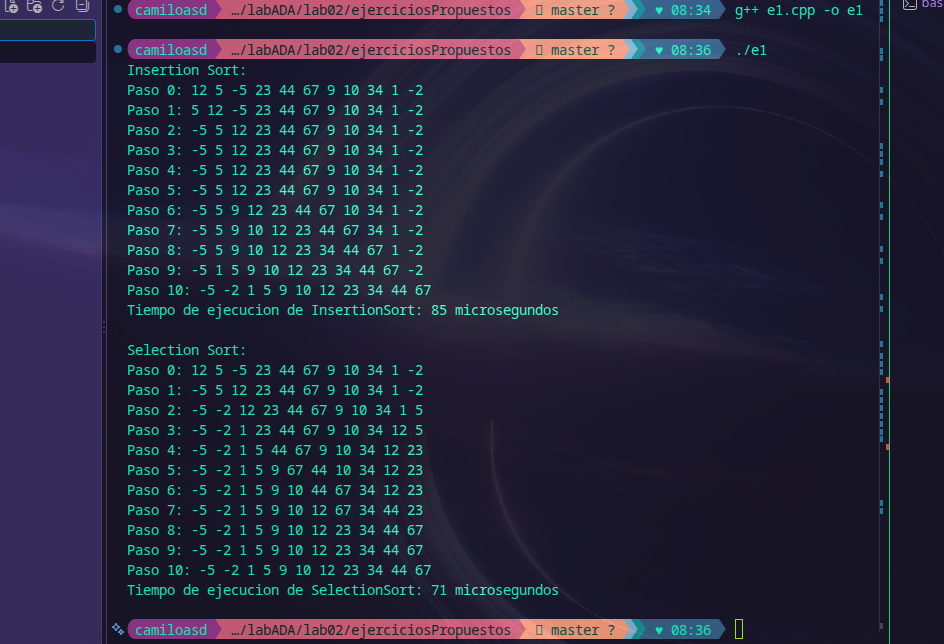
\includegraphics[width=0.8\textwidth]{img/e1.png}
    \caption{Ejecución de e1.cpp}
    \label{fig:diagrama}
    \end{figure}

	\subsection{Ejercicio 2}

        Implementa el algoritmo Insertion Sort para ordenar una lista de $n$ nombres ingresados por el usuario. Analiza su comportamiento con una lista ya ordenada, una lista en orden inverso y una lista aleatoria. ¿Cómo cambia el tiempo de ejecución?
    
    \lstinputlisting[language=c++, caption={Ejercicio 02: InsertionSort en una lista de n nombres y comparaciones con otras listas.},numbers=left,]{../ejerciciosPropuestos/e2.cpp}

    \begin{itemize}
        \item Como el usuario ingresará datos, usamos <Vector> para arrays dinamicos. En escencia el algoritmo se encuentra en las lineas 7 - 18, insertionSortNombres(vector<string>\& arr) compara elementos y los reordena, desplazando elementos mayores hacia la izquierda para hacer
		espacio a los elementos que se colocarán en sus lugares.  
    \end{itemize}

    \begin{figure}[H]
    \centering
    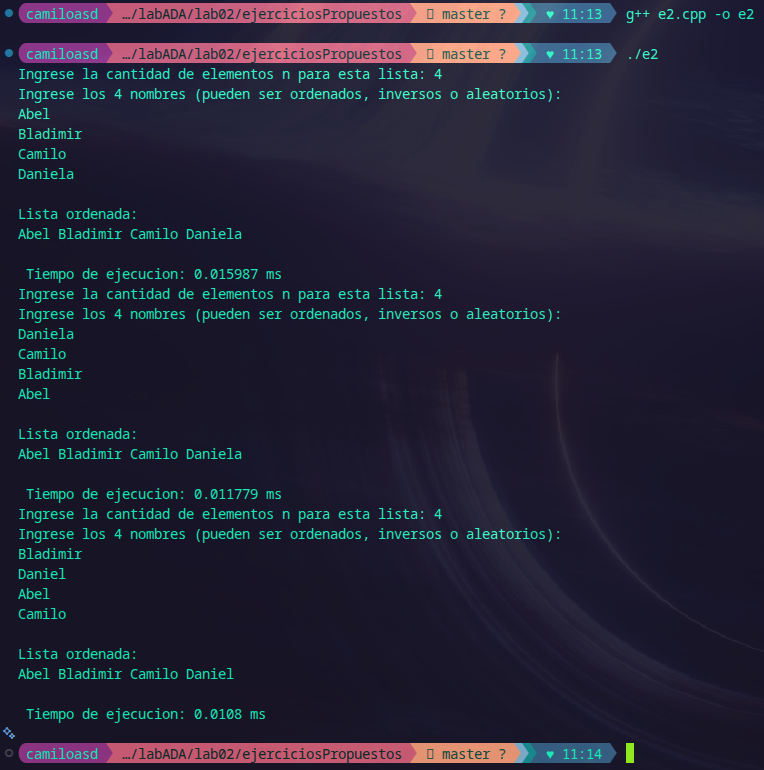
\includegraphics[width=0.9\textwidth]{img/e2.png}
    \caption{Ejecución de e2.cpp}
    \label{fig:diagrama}
    \end{figure}

	\begin {itemize}
		\item Viendo la comparación de las 3 listas, quien demora menos tiempo es la lista desordenada, lo cual es contraintuitivo ya que una lista ordenada debería tomar menos tiempo. Esto es debido a que
		las condiciones del hardware pueden afectar, además las comparaciones son consecutivas, no simultáneas, por lo que para pequeños datos (3 strings) esta comparación no muestra realmente las complejidades 
		temporales del algortimo.
	\end{itemize}

	\subsection{Ejercicio 3}

		Implementa el algoritmo Selection Sort sobre un arreglo de números flotantes. Muestra el número de comparaciones e intercambios realizados.
    
		\lstinputlisting[language=c++, caption={Ejercicio 03: SelectionSort sobre arreglo de numeros float.},numbers=left,]{../ejerciciosPropuestos/e3.cpp}

    \begin{itemize}
        \item En las líneas 6 – 24, la función selectionSortFloats asume inicialmente que el primer elemento de la parte aún no ordenada es el mínimo (minIdx = i). Luego recorre los elementos restantes y, en cada comparación, actualiza minIdx si encuentra un valor 
		menor. Al finalizar el recorrido, intercambia el mínimo encontrado con el elemento de la posición i, únicamente si están en posiciones diferentes. El programa usa contadores para registrar el número de comparaciones y de intercambios realizados.
    \end{itemize}

    \begin{figure}[H]
    \centering
    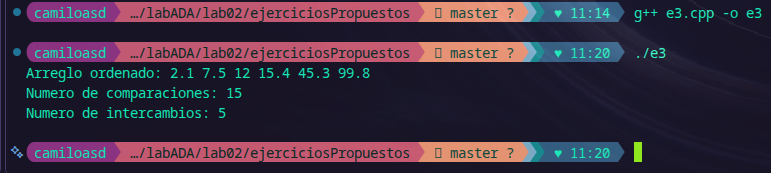
\includegraphics[width=0.8\textwidth]{img/e3.png}
    \caption{Ejecución de e3.cpp}
    \label{fig:diagrama}
    \end{figure}

	\subsection{Ejercicio 4}

		Crea una función que reciba un arreglo y un tipo de ordenamiento (insertion o selection) y aplique el algoritmo correspondiente. Evalúa el rendimiento con 1000, 5000 y 10000 elementos aleatorios.    
		\lstinputlisting[language=c++, caption={Ejercio 04: Función que recibe el tipo de ordenamiento.},numbers=left,]{../ejerciciosPropuestos/e4.cpp}

    \begin{itemize}
        \item Se usan las librerías cstdlib y algorithm para generar y colocar números pseudoaleatorios en los vectores. En main() se crea un vector con los tamaños 1000, 5000 y 10 000. Para cada tamaño, se crea un vector de enteros y se llena con valores entre 0 y 99999. Después se llama a evaluarOrdenamiento() dos veces: una para 
		Insertion Sort y otra para Selection Sort. Cada algoritmo recibe una copia del mismo vector original, permitiendo comparar sus tiempos de ejecución de manera justa.
    \end{itemize}

    \begin{figure}[H]
    \centering
    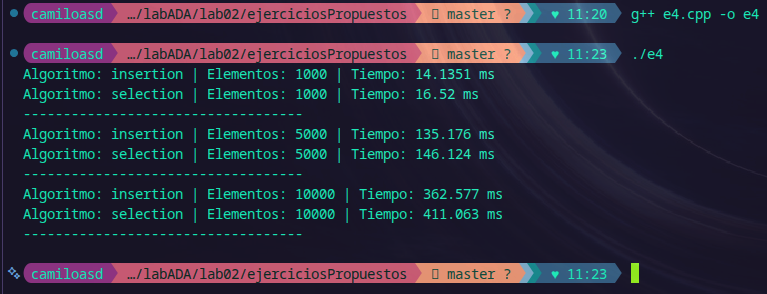
\includegraphics[width=0.8\textwidth]{img/e4.png}
    \caption{Ejecución de e4.cpp}
    \label{fig:diagrama}
    \end{figure}
	
	\subsection{Ejercicio 5}
		Desarrollen una aplicación en C++ que permita ordenar una lista de elementos sobre una temática libre elegida por el estudiante (en este caso, libros). Cada elemento debe contener al menos los siguientes atributos:
		\begin{itemize}
			\item Un identificador o código (string o entero).
			\item Un nombre o título (string).
			\item Un valor numérico que sirva como criterio de ordenamiento (número de páginas).
		\end{itemize}

		\noindent\textbf{Pasos a seguir:}
		\begin{itemize}
			\item Definir la temática y la estructura de los datos.
			\item Cargar los datos dinámicamente desde un archivo \texttt{.txt}.
			\item Ordenar los elementos de mayor a menor según el valor numérico, usando Insertion Sort y Selection Sort.
			\item Implementar contadores para las comparaciones realizadas y los intercambios efectuados.
			\item Medir el tiempo de ejecución.
			\item Exportar la lista ordenada a un archivo \texttt{.csv}.
		\end{itemize}

		\lstinputlisting[language=c++, caption={Ejercio 05: Creación de aplicación que ordena una lista de libros por número de páginas.},numbers=left,]{../ejerciciosPropuestos/e5.cpp}

    \begin{itemize}
        \item Lee los libros almacenados en libros.txt, obteniendo de cada uno su
  código, título y cantidad de páginas. Luego crea dos copias de la misma lista para
  ordenarlas de forma descendente según el número de páginas: una mediante Insertion
  Sort y otra mediante Selection Sort. Durante cada ordenamiento, registra la cantidad
  de comparaciones, los movimientos o intercambios realizados y el tiempo de ejecución.
  Después muestra estos resultados en pantalla para comparar ambos algoritmos y,
  finalmente, guarda la lista ordenada por Insertion Sort en el archivo
  libros\_ordenados.csv.

    \end{itemize}

    \begin{figure}[H]
    \centering
    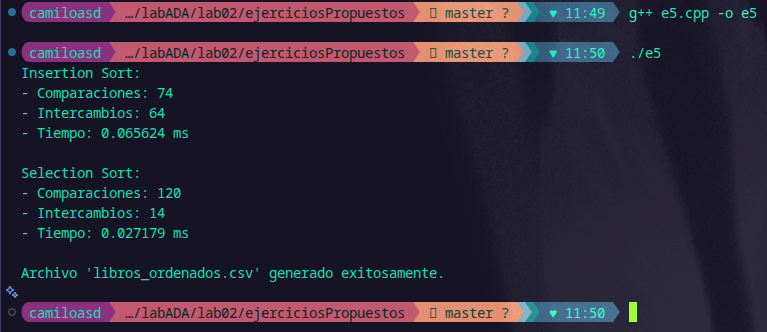
\includegraphics[width=0.95\textwidth]{img/e5(1).png}
    \caption{Ejecución de e5.cpp}
    \label{fig:diagrama}
    \end{figure}

   \begin{figure}[H]
    \centering
    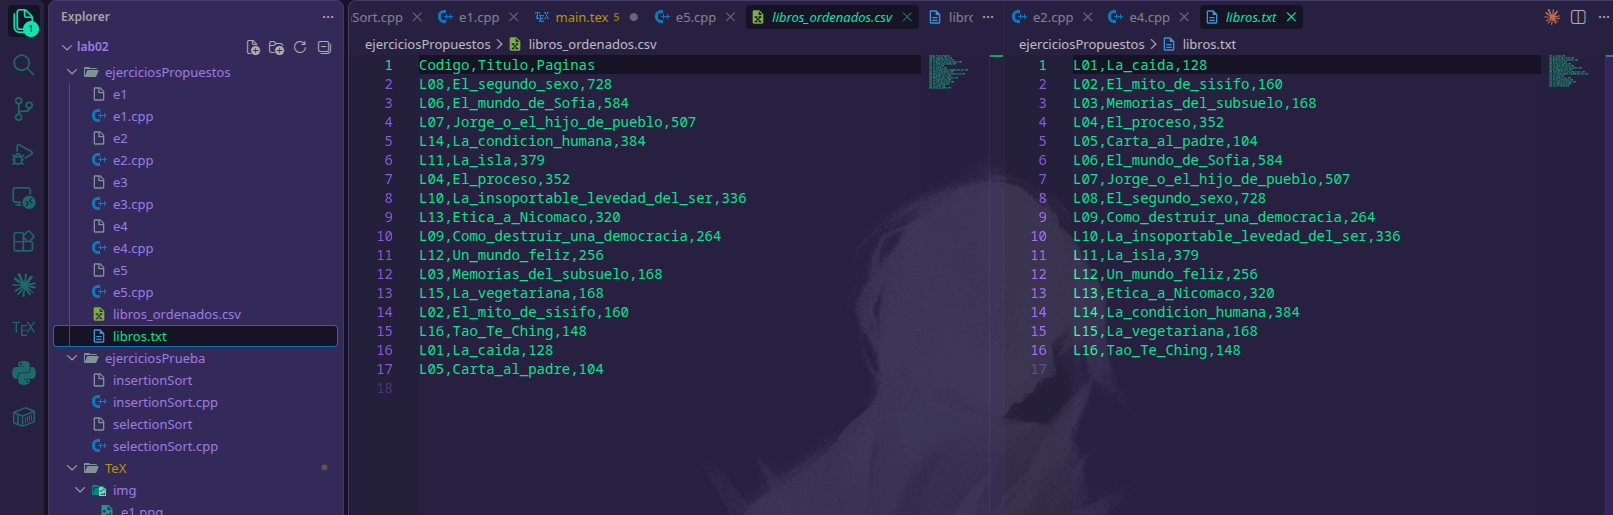
\includegraphics[width=0.95\textwidth]{img/e5(2).png}
    \caption{Comparacion de .csv (ordenado por n° de páginas) vs .txt (desordenado por n° de páginas)}
    \label{fig:diagrama}
    \end{figure}


	\section{Cuestionario}

		\begin{enumerate}

			\item Explica con tus propias palabras: ¿cuál de los dos algoritmos es más eficiente si la lista ya está ordenada? ¿Por qué? Usa un ejemplo distinto al visto en clase.
			
			Si la lista ya está ordenada, Insertion Sort es más eficiente. Esto se debe
			a que, al revisar cada elemento, observa que ya está en la posición correcta y no
			necesita desplazar elementos. Por ejemplo, si se tiene la lista de edades $\{18,
			20, 22, 25, 30\}$, Insertion Sort solo compara cada edad con la anterior y
			continúa, porque no encuentra ningún valor que deba mover. En cambio, Selection
			Sort sigue buscando el menor elemento en toda la parte no ordenada, aunque los
			datos ya estén ordenados.

			\item En tus palabras, ¿qué significa que un algoritmo sea "in-place"? Da un
	ejemplo de tu vida cotidiana donde "ordenar sin usar espacio extra" tendría
	sentido.

			Que un algoritmo sea \textit{in-place} significa que ordena los datos usando
			muy poca memoria adicional, normalmente sin crear otra lista del mismo tamaño. Por
			ejemplo, al ordenar libros en un estante, se puede tomar un libro y cambiarlo de
			posición con otro dentro del mismo estante, sin necesitar una segunda estantería
			para guardar todos los libros temporalmente.

			\item ¿Por qué se dice que Selection Sort no es estable? Describe un caso concreto
	(puede ser inventado por ti) donde eso cause un problema real.
			
			Se dice que Selection Sort no es estable porque puede cambiar el orden
			original de dos elementos que tienen la misma clave de comparación. Por ejemplo,
			si se ordenan libros por cantidad de páginas y se tienen los libros
			\texttt{A(200)}, \texttt{B(150)} y \texttt{C(200)}, al hacer un intercambio, los
			libros A y C, que tienen la misma cantidad de páginas, podrían quedar en un orden
			diferente al original. Esto sería un problema si el orden inicial representara
			otro criterio importante, como la fecha de publicación o el orden en que los
			libros fueron registrados.

			\item ¿Qué parte te costó más entender entre Insertion Sort y Selection Sort, y cómo
	la resolviste?
			
			La parte que más me costó entender fue la diferencia entre los
			desplazamientos de Insertion Sort y los intercambios de Selection Sort. Lo resolví
			siguiendo manualmente una lista pequeña y observando qué ocurría en cada
			iteración. Así comprendí que Insertion Sort mueve elementos para insertar uno en
			su posición correcta, mientras que Selection Sort busca el menor o mayor elemento
			y realiza un intercambio al final de cada pasada.

			\item Si tuvieras que explicarle a un compañero que faltó a la práctica cómo
	optimizar uno de estos dos algoritmos, ¿qué le dirías? 
			
			Para optimizar Insertion Sort, le diría a un compañero que es conveniente
			usarlo cuando la lista está ordenada o casi ordenada, porque en esos casos realiza
			pocos desplazamientos y puede ser rápido. Sin embargo, para listas muy grandes y
			desordenadas, recomendaría utilizar algoritmos más eficientes, como Merge Sort o
			Quick Sort, ya que Insertion Sort y Selection Sort tienen un tiempo de ejecución
			aproximado de $O(n^2)$.
		\end{enumerate}

	\section{Conclusiones}

	\begin{itemize}
		\item Se comprobó que Insertion Sort y Selection Sort permiten ordenar datos
		correctamente, pero su rendimiento puede variar según el orden inicial de los
		elementos.

		\item Insertion Sort resulta más conveniente cuando los datos ya están ordenados o
		casi ordenados, debido a que requiere menos desplazamientos.

		\item Selection Sort realiza una cantidad fija de comparaciones para un mismo
		tamaño de lista, aunque esta ya se encuentre ordenada; sin embargo, normalmente
		realiza pocos intercambios.

		\item Ambos algoritmos tienen una complejidad aproximada de $O(n^2)$, por lo que
		no son los más recomendables para listas muy grandes.

		\item La práctica permitió comprender cómo medir comparaciones, movimientos e
		tiempo de ejecución para evaluar el comportamiento de un algoritmo de
		ordenamiento.
	\end{itemize}

	%\begin{itemize}	
	%	\item Se creo el archivo \textbf{.gitignore} para no considerar los archivos %\textbf{*.class} que son innecesarios hacer seguimiento.
	%\end{itemize}
	%\begin{lstlisting}[language=bash,caption={Creando .gitignore}]
	%	$ vim lab01/.gitignore
	%\end{lstlisting}
	%\begin{lstlisting}[language=bash,caption={lab01/.gitignore}]
	%	*.class
	%\end{lstlisting}
	%\begin{lstlisting}[language=bash,caption={Commit: Creando .gitignore para archivos *.class}]
	%	$ git add .
	%	$ git commit -m "Creando .gitignore para archivos *.class"			
	%	$ git push -u origin main
	%\end{lstlisting}
	
	%\begin{lstlisting}[language=bash,caption={Creando .gitignore}]
	%	$ vim lab01/Insertion.java
	%\end{lstlisting}
	
    
%\clearpage
%\bibliographystyle{apalike}
%\bibliographystyle{IEEEtranN}
%\bibliography{bibliography}
			
\end{document}\noindent\textbf{Enunciado:} 